%!TeX root = ../main.tex
\section*{Lecture 17, 10/04/2018}
Today: The large-$N$ limit.
This has something to do with the AdS/CTF correspondence.
\me{Some historical discussion happened.}

Recall that in $SU(N)$ QCD there is no universally available expansion parameter, becasue the way renormalization works fixes a \emph{physical} scale $\Lambda_{QCD}$.
Therefore there is no universally available expansion parameter.
t'Hooft had the idea to deal with this by expanding in $1/N$, where $N$ is the rank of the gauge group.
It turns out that this can be made to work!
It's also relevant to statistical mechanics: H.E.~Stanley wrote a PRL paper (so it's short and readable) about trying to understand $O(n)$ spin models as $n \to \infty$.
Recall that $n = 0$ describes self-avoiding walks, $n =1$ is the Ising model, $n = 2$ is XY, and $n = 3$ is the Heisenberg model.

Similarly, t'Hooft has a paper on large $N$ QCD in $1+1$ dimensions, which someone presented in discussion.
We warm up with a simpler example, related to the $(1+1)$-dimensional Thirring model:
\[
S_T = \int d^2x \bar \psi i \slashed \partial \psi - g_T \bar (\psi \psi_\mu \psi)^2. 
\]
We previously sovled this model via bosonization.

Consider the similar Gross-Neveu model
\[
S_{GN} = \int d^2 x \bar \psi i \slashed d \psi - \frac{g}{2} (\bar \psi \psi)^2,
\]
where $\psi = \psi^a$, $a = 1, \dots , N$ is a Dirac spinor.
This model has a naive global $SU(N)$ symmetry; it can be extended to $SO(2N)$ by rotating particles and antiparticles into each other, but we don't need to do this.
Notice that for both theories the coupling constant is dimensionless.
This is a sort of baby QCD with only a matter sector.

This theory has a discrete chiral $\mathbb{Z}_2$ symmetry via $\psi \to - \gamma_3 \psi$, $\bar \psi \to - \bar \psi \gamma_3$.
There's no classical mass, but \me{something about asymptotic freedom.
I think that it will turn out to be so.}

In the $N \to \infty$ limit where there are no $1/N$ corrections, the propagator is just $\delta_{ab}$, and we can think about vertices splitting apart:
\[
\feynmandiagram[horizontal = a to b, baseline = (e.base)]{
    a [particle = $a$] --[fermion] e --[fermion] b [particle = $a$],
    c [particle = $b$] --[fermion] e --[fermion] d [particle = $b$]
};
=
\feynmandiagram[vertical = e1 to e2, baseline = (e1.base)]{
    a [particle = $a$] --[fermion] e1 --[fermion] b [particle = $a$],
    c [particle = $b$] --[fermion] e2 --[fermion] d [particle = $b$],
    e1 -- [ghost] e2
};
\]
Now the expansion of an $a, \bar a \to b , \bar b$ scattering looks like
\begin{center}
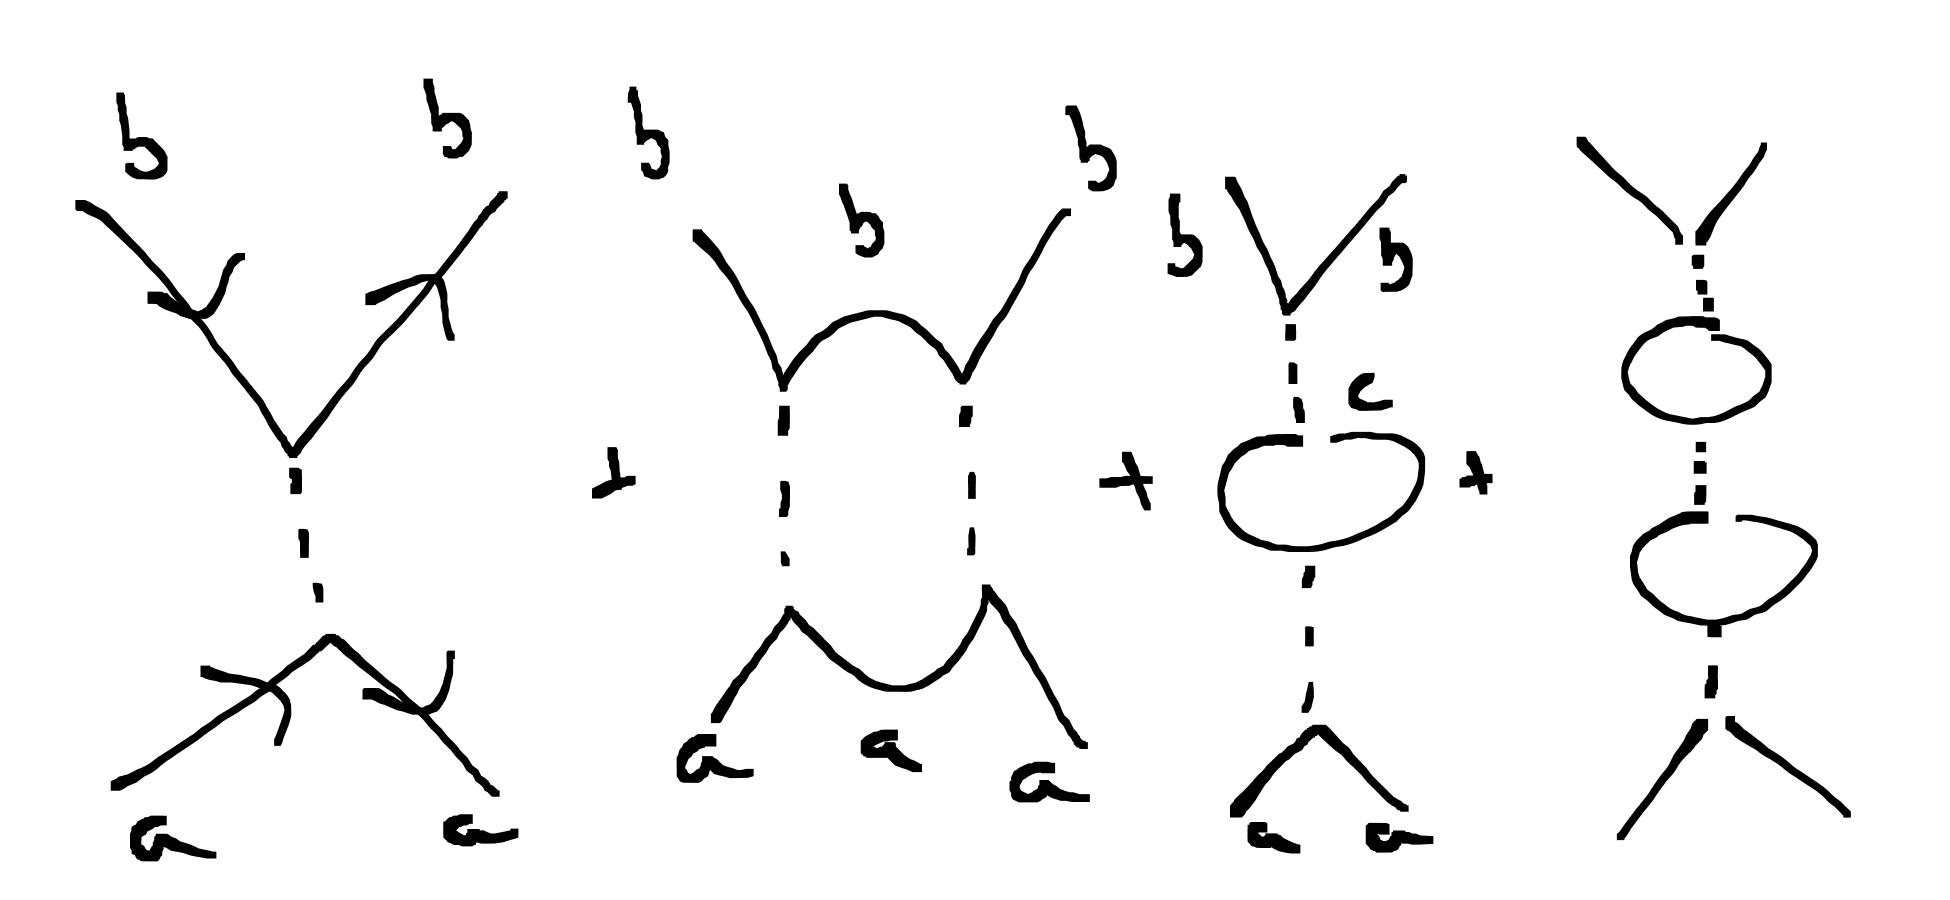
\includegraphics{fig/largeNexample.png}
\end{center}
\me{This \emph{could} be done in tikzFeynman but would probably require manual vertex placement.
I did not feel like dealing with that.}
Note that these are just representative terms.
When you take the traces in the loops these terms are order $g$, $g^2$, $g^2 n$, and $g^3 N^2$ respectively.
This will not work as $N \to \infty$.
We need a new coupling $\lambda^2 = gN$, which is fixed as $N \to \infty$.
The expansion terms above are now $\lambda^2/N$, $\lambda^4/N^2$, $\lambda^4/N$, $\lambda^6/N$, so they can converge.

We can then rewrite the action as
\[
\int d^2 x \bar \psi i \slashed \partial \psi - \frac{\lambda^2}{2 N}(\bar \psi \psi)^2.
\]
You might think that this will be free in the $N \to \infty$ limit, but this doesn't quite work, because there's an $N$ in the first term.

To deal with this question, introduce an auxiliary field
\[
\sigma = \frac{\lambda}{N} \bar \psi \psi.
\]
We can now integrate out $\bar \psi$ and $\psi$ to get an effective potential
\[
-i V(\sigma_0) = - i \frac{N}{2 \lambda^2} \sigma^2 - N \sum_{r=1}^\infty \frac{1}{2r} \tr \int \frac{d^2 p}{(2 \pi)^2} \left(\frac{- \slashed p \sigma}{p^3} \right)^{2r},
\]
so that
\[
V = \frac{N}{2 \lambda^2} \sigma - N \int \frac{d^2 p}{(2 \pi)^2} \log\left( 1 + \frac{\sigma_0}{\me{??}} \right).
\]
This gives an effective mass for $\psi$ and breaks the chiral symmetry.

\me{I missed a portion of the following discussion.}
$\sigma$ is a \emph{master field.}
It is possible to associate $1/N \sim \hbar$ and get a classical limit.

\subsection*{More systematic approach to large $N$}
Consider a generic QFT of some fields $M$, which we take to be matrices in some simple Lie group, say $U(N)$.
\me{There was a comment about choosing them Hermitian, which would mean that they're in the Lie algebra.
Since this is field theory, those are the same thing.}
The action is of the form
\[
S = \int \tr \left[ (\partial M)^2 + \highlight{M^2 + M^3 + \cdots} \right]
\]
with the \highlight{highlighted terms} grouped together to give a potential $V(M)$.
Because the matrices have \emph{two} indices, the propagators have two edges and the Feynman diagrams are \emph{ribbon} graphs.

Notice that the propagators contribute $g^2$, the vertices contribute $1/g^2$, and the loops contribute an $N$ from the trace.
Therefore a general diagram scales as
\[
(g^2)^{P - V} N^L = (g^2 N)^{P - V} N^{V - P + L}
\]
where $P$ is the number of propagators (edges), $V$ the number of vertices, and $L$ the number of loops.
The second term above is $(1/N)^{2g -2}$, where $g$ is the genus of the ribbon graph.
This is one way to motivate string theory: we have a perturbative expansion over surfaces.